\documentclass{ximera}

%% You can put user macros here
%% However, you cannot make new environments

\listfiles

\graphicspath{{./}{firstExample/}{secondExample/}}

\usepackage{tikz}
\usepackage{tkz-euclide}
\usepackage{tikz-3dplot}
\usepackage{tikz-cd}
\usetikzlibrary{shapes.geometric}
\usetikzlibrary{arrows}
\usetikzlibrary{decorations.pathmorphing,patterns}
\usetkzobj{all}
\pgfplotsset{compat=1.13} % prevents compile error.

\renewcommand{\vec}[1]{\mathbf{#1}}
\newcommand{\RR}{\mathbb{R}}
\newcommand{\dfn}{\textit}
\newcommand{\dotp}{\cdot}
\newcommand{\id}{\text{id}}
\newcommand\norm[1]{\left\lVert#1\right\rVert}
 
\newtheorem{general}{Generalization}
\newtheorem{initprob}{Exploration Problem}

\tikzstyle geometryDiagrams=[ultra thick,color=blue!50!black]

\usepackage{mathtools}

\title{8.3 Solution of Initial Value Problems}%\label{Module 7-ADEF}

\begin{document}

\begin{abstract}
We demonstrate how Laplace transforms can be used to solve constant coefficient second order initial value problems.
\end{abstract}

\maketitle

\section*{Solution of Initial Value Problems}

\subsection*{Laplace Transforms of Derivatives}

In the rest of this chapter we'll use the Laplace transform to solve
initial value problems for constant coefficient second order
equations. To do this, we must know how the Laplace transform of
 $f'$ is related to the Laplace transform of $f$. The
next theorem answers this question.

\begin{theorem}\label{thmtype:8.3.1}
 Suppose $f$ is continuous
on $[0,\infty)$ and of exponential order $s_0$, and $f'$ is piecewise
continuous on $[0,\infty).$  Then $f$ and $f'$ have Laplace transforms for
$s > s_0,$ and
\begin{equation}\label{eq:8.3.1}
{\cal L}(f')=s {\cal L}(f)-f(0).
\end{equation}
\end{theorem}

\begin{proof}

We know from Theorem~8.1.6 that ${\cal L}(f)$ is defined for
$s>s_0$.
We first consider the case where $f'$ is continuous on $[0,\infty)$.
Integration by parts yields
\begin{equation}\label{eq:8.3.2}
\begin{array}{ccl}
\int^T_0 e^{-st}f'(t)\,dt &=& e^{-st}f(t)\Big|^T_0+s
\int^T_0e^{-st}f(t)\,dt\\
&=& e^{-sT}f(T)-f(0)+s\int^T_0 e^{-st}f(t)\,dt
\end{array}
\end{equation}
for any $T>0$. Since $f$ is of exponential order $s_0$,
 $\lim_{T\to \infty}e^{-sT}f(T)=0$ and the last integral in
\eqref{eq:8.3.2} converges as $T\to\infty$ if $s> s_0$. Therefore
\begin{eqnarray*}
\int^\infty_0 e^{-st}f'(t)\,dt&=&-f(0)+s\int^\infty_0
e^{-st}f(t)\,dt\\ &=&-f(0)+s{\cal L}(f),
\end{eqnarray*}
which proves  \eqref{eq:8.3.1}.
Now  suppose     $T>0$  and  $f'$  is  only piecewise continuous on
$[0,T]$, with discontinuities  at $t_1 <  t_2 <\cdots <  t_{n-1}$. For
convenience,  let  $t_0=0$  and  $t_n=T$.  Integrating by parts yields
\begin{eqnarray*}       \int^{t_i}_{t_{i-1}}e^{-st}f'(t)\,dt       &=&
e^{-st}f(t)\Big|^{t_i}_{t_{i-1}}+s\int^{t_i}_{t_{i-1}}e^{-st}f(t)\,dt\\
&=&                         e^{-st_i}                          f(t_i)-
e^{-st_{i-1}}f(t_{i-1})+s\int^{t_i}_{t_{i-1}}e^{-st}f(t)\,dt.
\end{eqnarray*} Summing both sides of this equation from $i=1$ to  $n$
and noting that
$$
\left(e^{-st_1}f(t_1)-e^{-st_0}f(t_0)\right)+\left(e^{-st_2}
f(t_2)-e^{-st_1}f(t_1)\right)
+\cdots+\left(e^{-st_N}f(t_N)-e^{-st_{N-1}}f(t_{N-1})\right)
$$
$$
=e^{-st_N}f(t_N)-e^{-st_0}f(t_0)=e^{-sT}f(T)-f(0)
$$
yields \eqref{eq:8.3.2}, so \eqref{eq:8.3.1} follows as before.
\end{proof}

\begin{example}\label{example:8.3.1}
 In Example~\ref{example:8.1.4} we saw that
$$
{\cal L}(\cos\omega t)=\frac{s}{s^2+\omega^2}.
$$
Applying  \eqref{eq:8.3.1} with $f(t)=\cos\omega t$ shows that
$$
{\cal L}(-\omega\sin\omega t)=s \frac{s}{s^2+\omega^2}-1=-
\frac{\omega^2}{s^2+\omega^2}.
$$
Therefore
$$
{\cal L}(\sin\omega t)=\frac{\omega}{s^2+\omega^2},
$$
which agrees with the corresponding  result obtained  in
\ref{example:8.1.4}.
\end{example}

%In Section~2.1 we showed 
At this point it is easy for us to check (do so!)
that the solution of the
initial value problem
\begin{equation}\label{eq:8.3.3}
y'=ay, \quad  y(0)=y_0,
\end{equation}
 is $y=y_0e^{at}$.
We'll now obtain this result by using the Laplace transform.

Let $Y(s)={\cal L}(y)$ be the Laplace transform of the unknown solution
of \eqref{eq:8.3.3}. Taking Laplace transforms of both sides of
\eqref{eq:8.3.3} yields
$$
{\cal L}(y')={\cal L}(ay),
$$
which, by Theorem~\ref{thmtype:8.3.1}, can be rewritten as
$$
s{\cal L}(y)-y(0)=a{\cal L}(y),
$$
or
$$
sY(s)-y_0=aY(s).
$$
Solving for $Y(s)$ yields
$$
Y(s)=\frac{y_0}{s-a},
$$
so
$$
y={\cal L}^{-1}(Y(s))={\cal L}^{-1}\left(\frac{y_0}{s-a}\right)=y_0{\cal
L}^{-1}\left(\frac{1}{s-a}\right)=y_0e^{at},
$$
which agrees with the known result.

We  need the next theorem to solve second order differential equations
using  the Laplace transform.

\begin{theorem}\label{thmtype:8.3.2}
Suppose $f$ and $f'$ are continuous on $[0,\infty)$ and of
exponential order $s_0,$ and that $f''$ is piecewise continuous on
$[0,\infty).$ Then $f$, $f'$, and $f''$ have Laplace transforms for $s
> s_0$,
\begin{equation}\label{eq:8.3.4}
{\cal L}(f')=s {\cal L}(f)-f(0),
\end{equation}
and
\begin{equation}\label{eq:8.3.5}
{\cal L}(f'')=s^2{\cal L}(f)-f'(0)-sf(0).
\end{equation}
\end{theorem}

\begin{proof}
Theorem~\ref{thmtype:8.3.1} implies that ${\cal L}(f')$ exists and
satisfies \eqref{eq:8.3.4} for $s>s_0$. To prove that ${\cal L}(f'')$
exists and satisfies \eqref{eq:8.3.5} for $s>s_0$, we first apply
Theorem~\ref{thmtype:8.3.1} to $g=f'$. Since $g$ satisfies the hypotheses
of Theorem~\ref{thmtype:8.3.1}, we conclude that ${\cal L}(g')$ is defined
and satisfies
$$
{\cal L}(g')=s{\cal L}(g)-g(0)
$$
for $s>s_0$. However, since $g'=f''$, this can be rewritten as
$$
{\cal L}(f'')=s{\cal L}(f')-f'(0).
$$
Substituting \eqref{eq:8.3.4} into this yields
\eqref{eq:8.3.5}.
\end{proof}

\subsection*{Solving Second Order Equations with the Laplace Transform}

We'll now use the Laplace transform to solve initial value problems
for  second order equations.

\begin{example}\label{example:8.3.2}
Use the Laplace transform to solve the initial value problem
\begin{equation}\label{eq:8.3.6}
y''-6y'+5y=3e^{2t},\quad y(0)=2, \quad   y'(0)=3.
\end{equation}
\begin{explanation}
Taking Laplace transforms of both sides of the differential equation
in \eqref{eq:8.3.6} yields
$$
{\cal L}(y''-6y'+5y)={\cal L}\left(3e^{2t}\right)=\frac{3}{s-2},
$$
which we rewrite as
\begin{equation}\label{eq:8.3.7}
{\cal L}(y'')-6{\cal L}(y')+5{\cal L}(y)=\frac{3}{s-2}.
\end{equation}
Now denote ${\cal L}(y)=Y(s)$. Theorem~\ref{thmtype:8.3.2} and the
initial conditions in \eqref{eq:8.3.6} imply that
$$
{\cal L}(y')=sY(s)-y(0)=sY(s)-2
$$
and
$$
{\cal L}(y'')=s^2Y(s)-y'(0)-sy(0)=s^2Y(s)-3-2s.
$$
Substituting from the last two equations into  \eqref{eq:8.3.7} yields
$$
\left(s^2Y(s)-3-2s\right)-6\left(sY(s)-2\right)+5Y(s)=\frac{3}{s-2}.
$$
Therefore
\begin{equation}\label{eq:8.3.8}
(s^2-6s+5)Y(s)=\frac{3}{s-2}+(3+2s)+6(-2),
\end{equation}
so
$$
(s-5)(s-1)Y(s)=\frac{3+(s-2)(2s-9)}{s-2},
$$
and
$$
Y(s)=\frac{3+(s-2)(2s-9)}{(s-2)(s-5)(s-1)}.
$$
Heaviside's method yields the partial fraction expansion
$$
Y(s)=-\frac{1}{s-2}+\frac{1}{2}\frac{1}{s-5}+\frac{5}{2}\frac{1}{s-1},
$$
and taking the inverse transform of this yields
$$
y=-e^{2t}+\frac{1}{2}e^{5t}+\frac{5}{2}e^t
$$
as the solution of  \eqref{eq:8.3.6}.
\end{explanation}
\end{example}

It isn't necessary to write all the steps that we used to obtain
\eqref{eq:8.3.8}. To see how to avoid this, let's apply the method of
Example~\ref{example:8.3.2} to the general initial value problem
\begin{equation}\label{eq:8.3.9}
ay''+by'+cy=f(t), \quad  y(0)=k_0,\quad y'(0)=k_1.
\end{equation}

Taking Laplace transforms of both sides of  the differential
equation in \eqref{eq:8.3.9} yields
\begin{equation}\label{eq:8.3.10}
a{\cal L}(y'')+b{\cal L}(y')+c{\cal L}(y)=F(s).
\end{equation}
Now let $Y(s)={\cal L}(y)$.  Theorem~\ref{thmtype:8.3.2} and the
initial conditions in \eqref{eq:8.3.9} imply that
$$
{\cal L}(y')=sY(s)-k_0\quad\mbox{and}\quad {\cal L}(y'')=s^2Y(s)-k_1-k_0s.
$$
Substituting these  into  \eqref{eq:8.3.10} yields
\begin{equation}\label{eq:8.3.11}
a\left(s^2Y(s)-k_1-k_0s\right)+b\left(sY(s)-k_0\right)+cY(s)=F(s).
\end{equation}
The coefficient of $Y(s)$ on the left is the characteristic
polynomial
$$
p(s)=as^2+bs+c
$$
of the complementary equation for \eqref{eq:8.3.9}. Using this and moving
the terms involving $k_0$ and $k_1$ to the right side of \eqref{eq:8.3.11}
yields
\begin{equation}\label{eq:8.3.12}
p(s)Y(s)=F(s)+a(k_1+k_0s)+bk_0.
\end{equation}
This equation corresponds to \eqref{eq:8.3.8} of Example~\ref{example:8.3.2}.
Having established the form of this equation in the general case, it
is preferable to go directly from the initial value problem to this
equation. You may find it easier to remember \eqref{eq:8.3.12} rewritten
as
\begin{equation} \label{eq:8.3.13}
p(s)Y(s)=F(s)+a\left(y'(0)+sy(0)\right)+by(0).
\end{equation}

\begin{example}\label{example:8.3.3}
 Use the Laplace transform to solve the
initial value problem
\begin{equation}\label{eq:8.3.14}
2y''+3y'+y=8e^{-2t}, \quad   y(0)=-4,  y'(0)=2.
\end{equation}

\begin{explanation}
The characteristic polynomial is
$$
p(s)=2s^2+3s+1=(2s+1)(s+1)
$$
 and
$$
F(s)={\cal L}(8e^{-2t})=\frac{8}{s+2},
$$
so \eqref{eq:8.3.13} becomes
$$
(2s+1)(s+1)Y(s)=\frac{8}{s+2}+2(2-4s)+3(-4).
$$
Solving  for $Y(s)$ yields
$$
Y(s)=\frac{4\left(1-(s+2)(s+1)\right)}{(s+1/2)(s+1)(s+2)}.
$$
Heaviside's method yields the partial fraction expansion
$$
Y(s)=\frac{4}{3}\frac{1}{s+1/2}-\frac{8}{s+1}+\frac{8}{3}\frac{1}{s+2},
$$
so the solution of  \eqref{eq:8.3.14} is
$$
y={\cal L}^{-1}(Y(s))=\frac{4}{3}e^{-t/2}-8e^{-t}+\frac{8}{3}e^{-2t}.
$$
%(Figure~\ref{figure:8.3.1}).

\begin{image}
 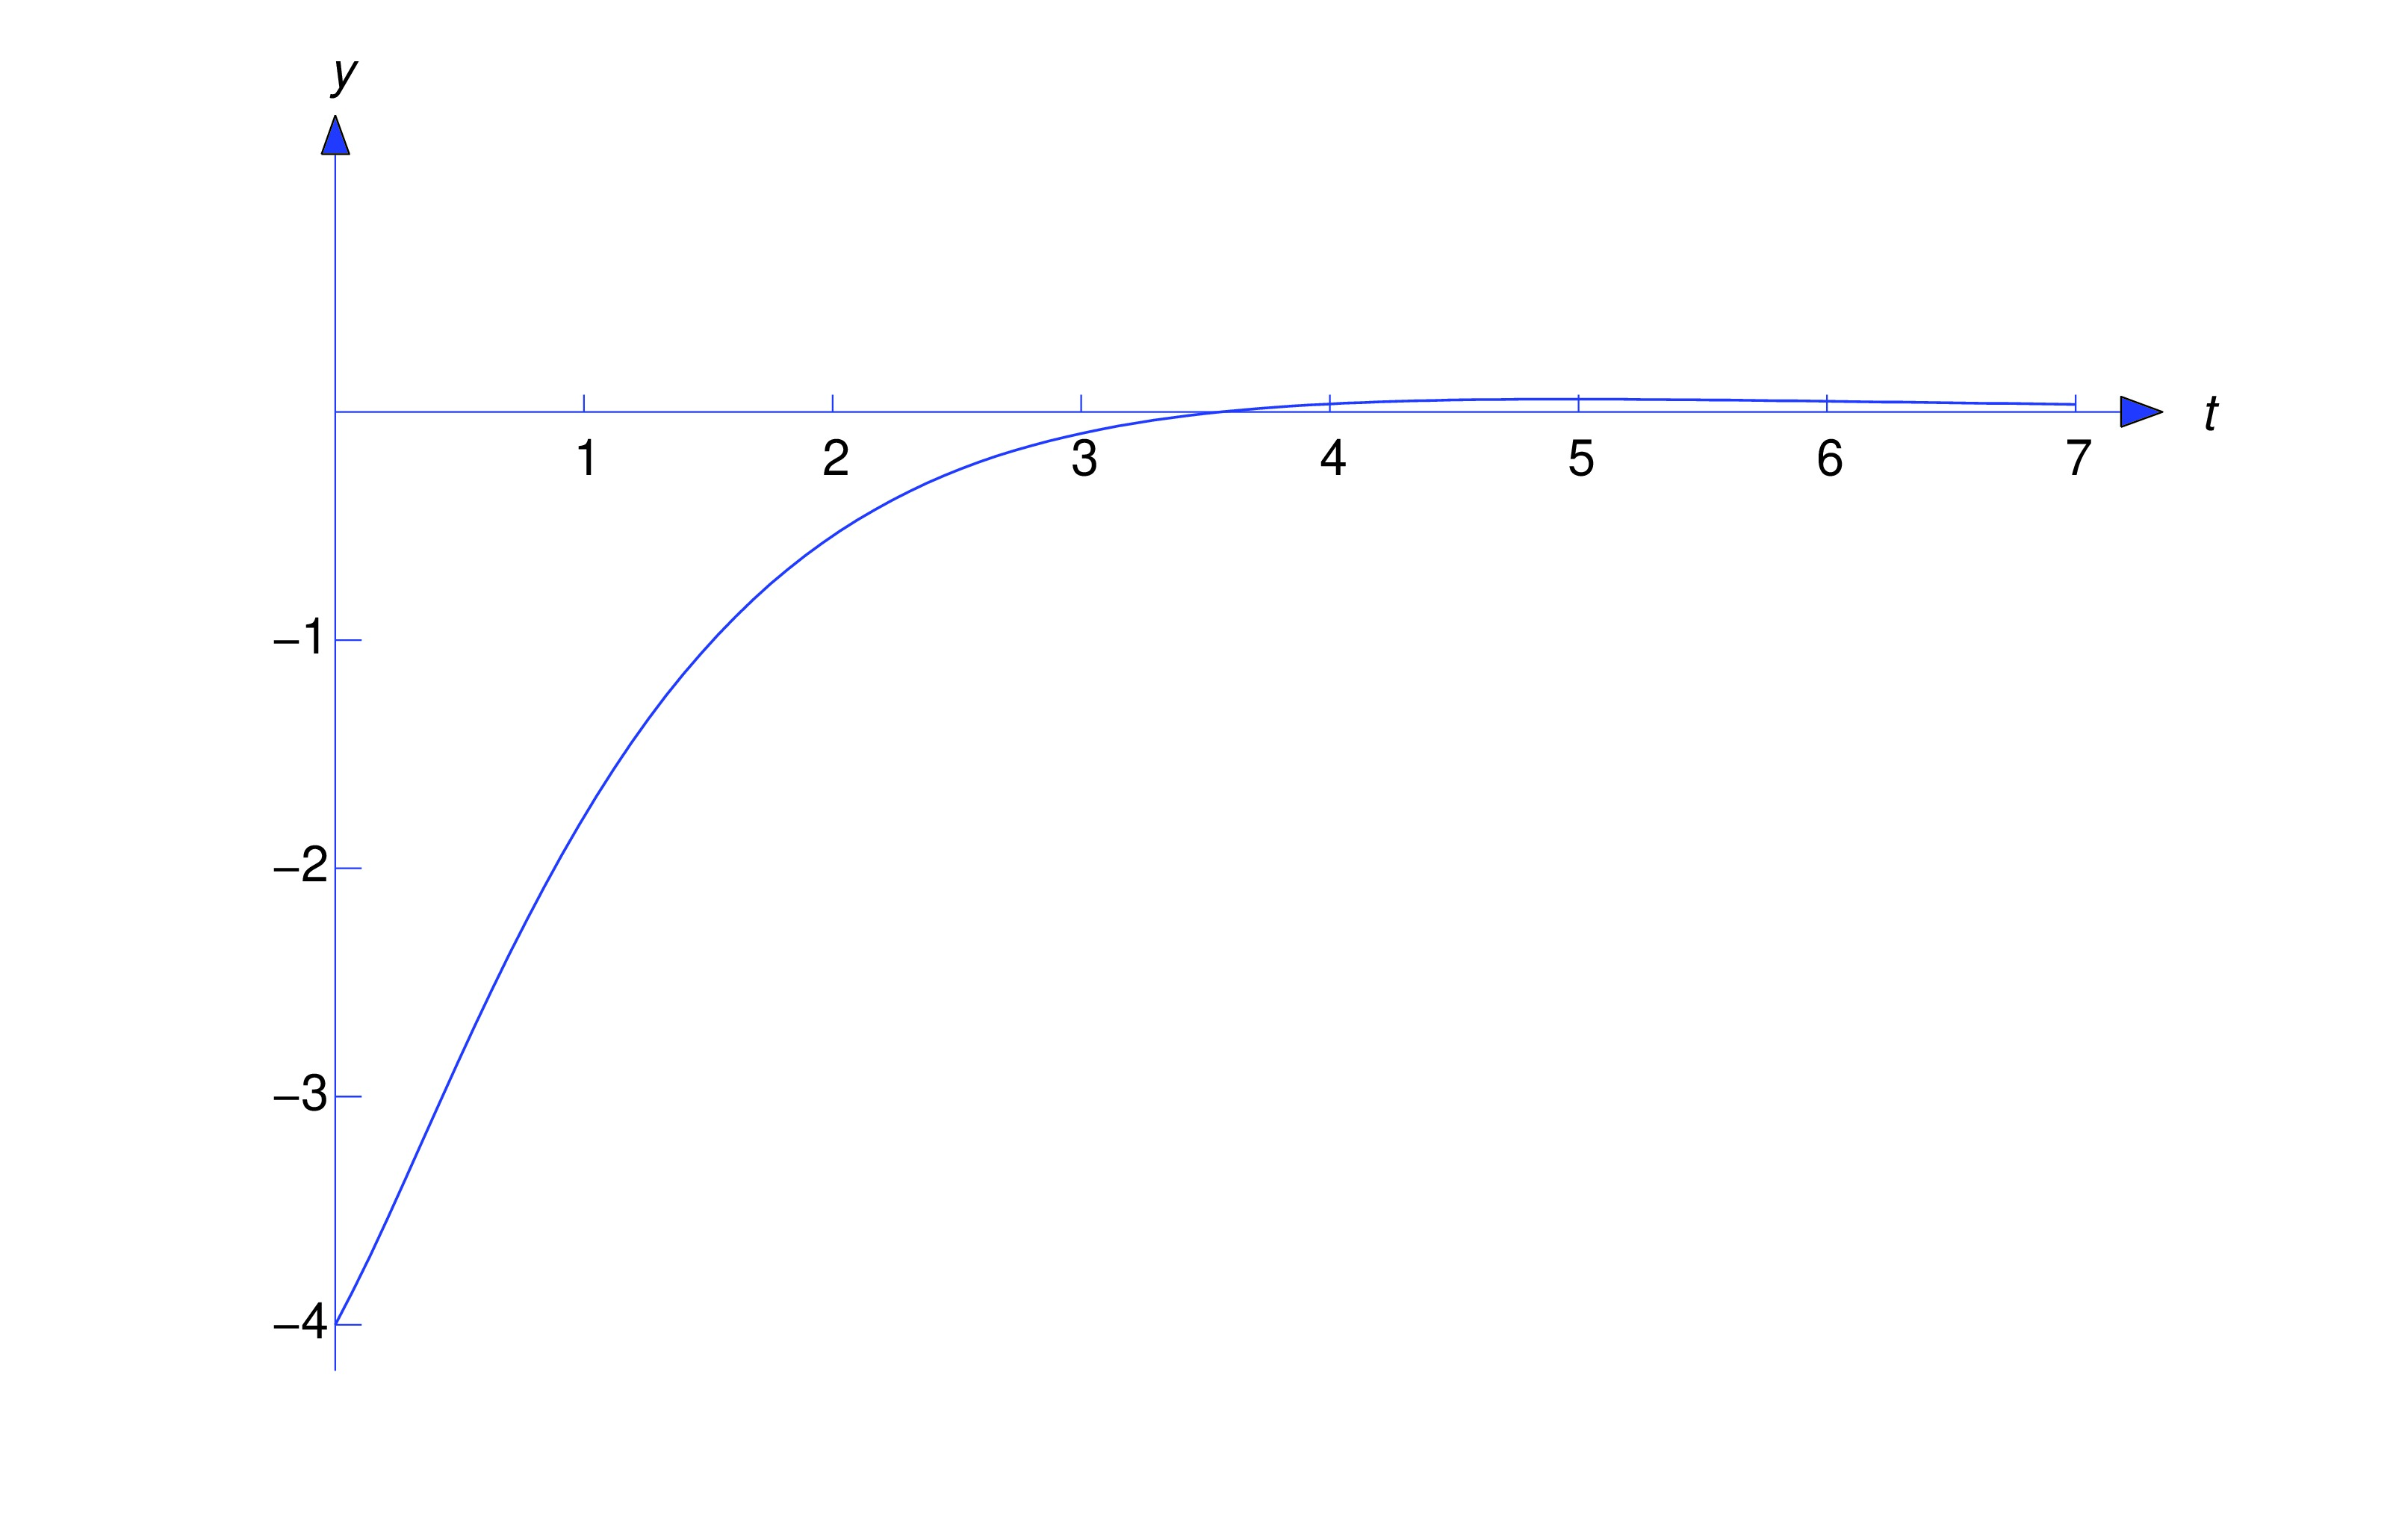
\includegraphics[height=1.5in]{fig080301.jpg}
 \end{image}
\end{explanation}
\end{example}

% \begin{figure}[htbp]
% \color{blue}
%   \begin{minipage}[b]{0.5\linewidth}
%     \centering
%   \scalebox{.65}{
%   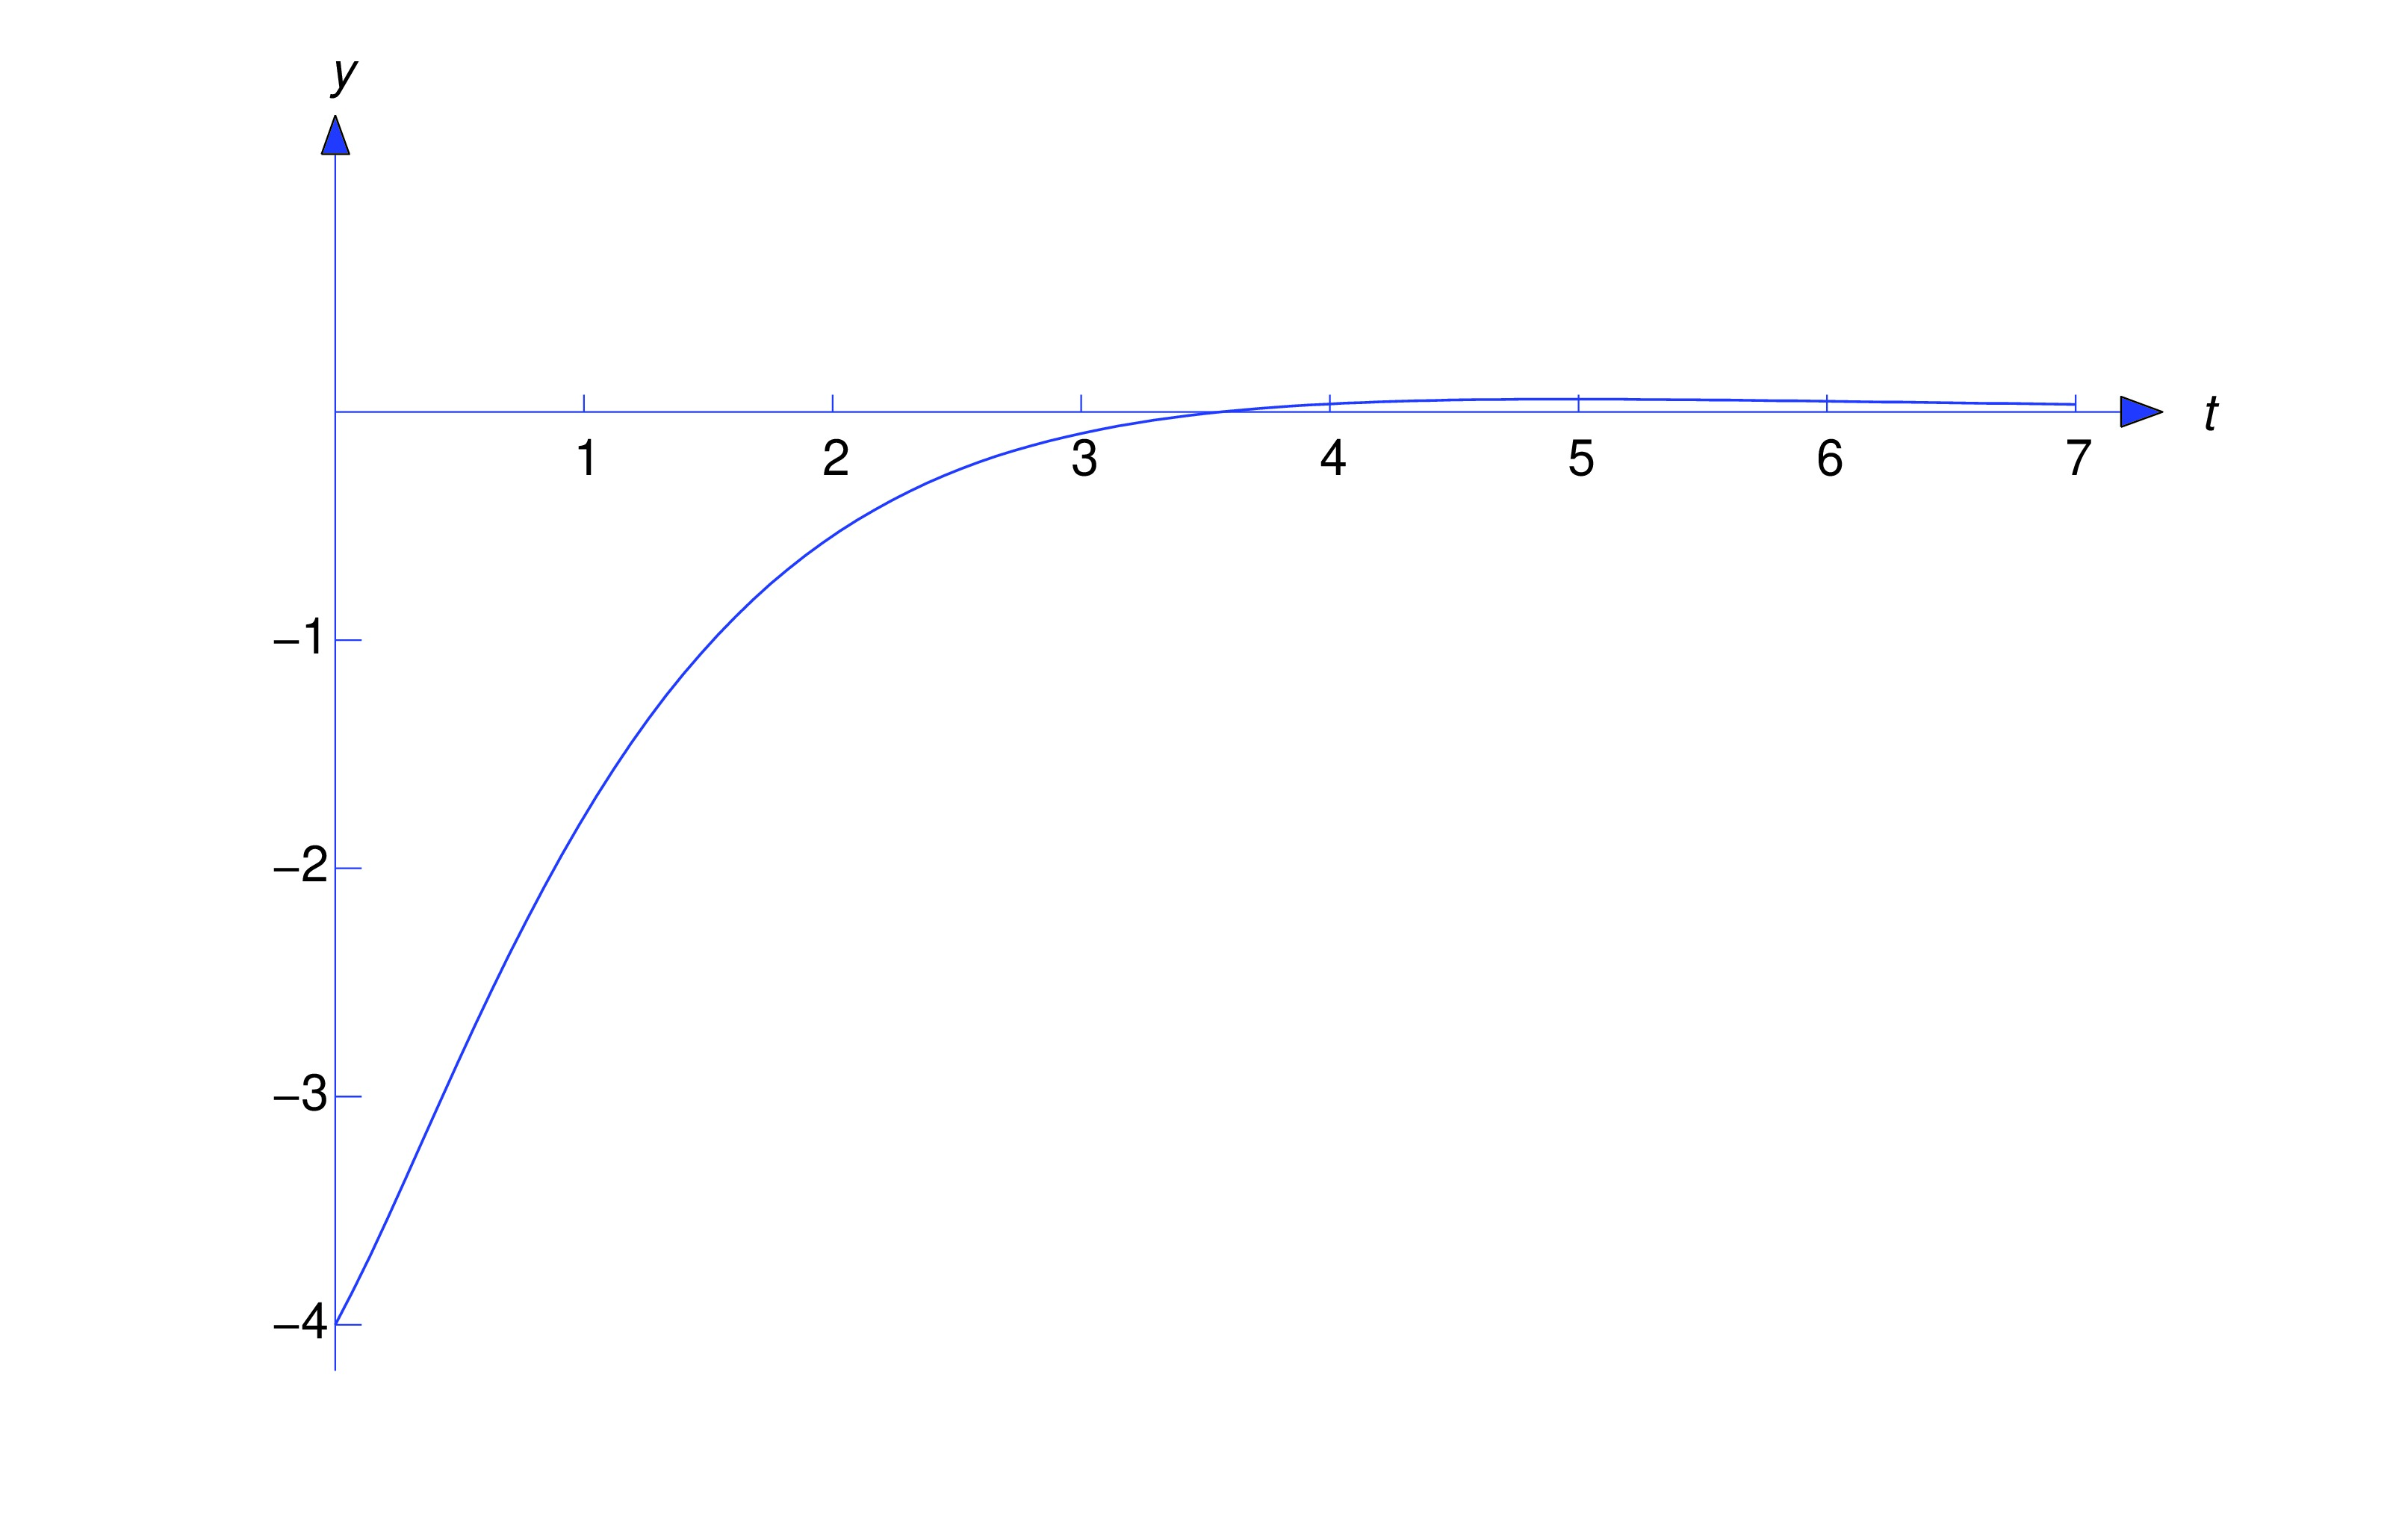
\includegraphics[bb=-78 148 689 643,width=5.67in,height=3.66in,keepaspectratio]{fig080301}}
% \caption{ $y=\dst{{4\over3}e^{-t/2}-8e^{-t}+{8\over3}e^{-2t}}$}
%   \label{figure:8.3.1}
% \end{minipage}
%   \begin{minipage}[b]{0.5\linewidth}
%     \centering
%   \scalebox{.65}{
%   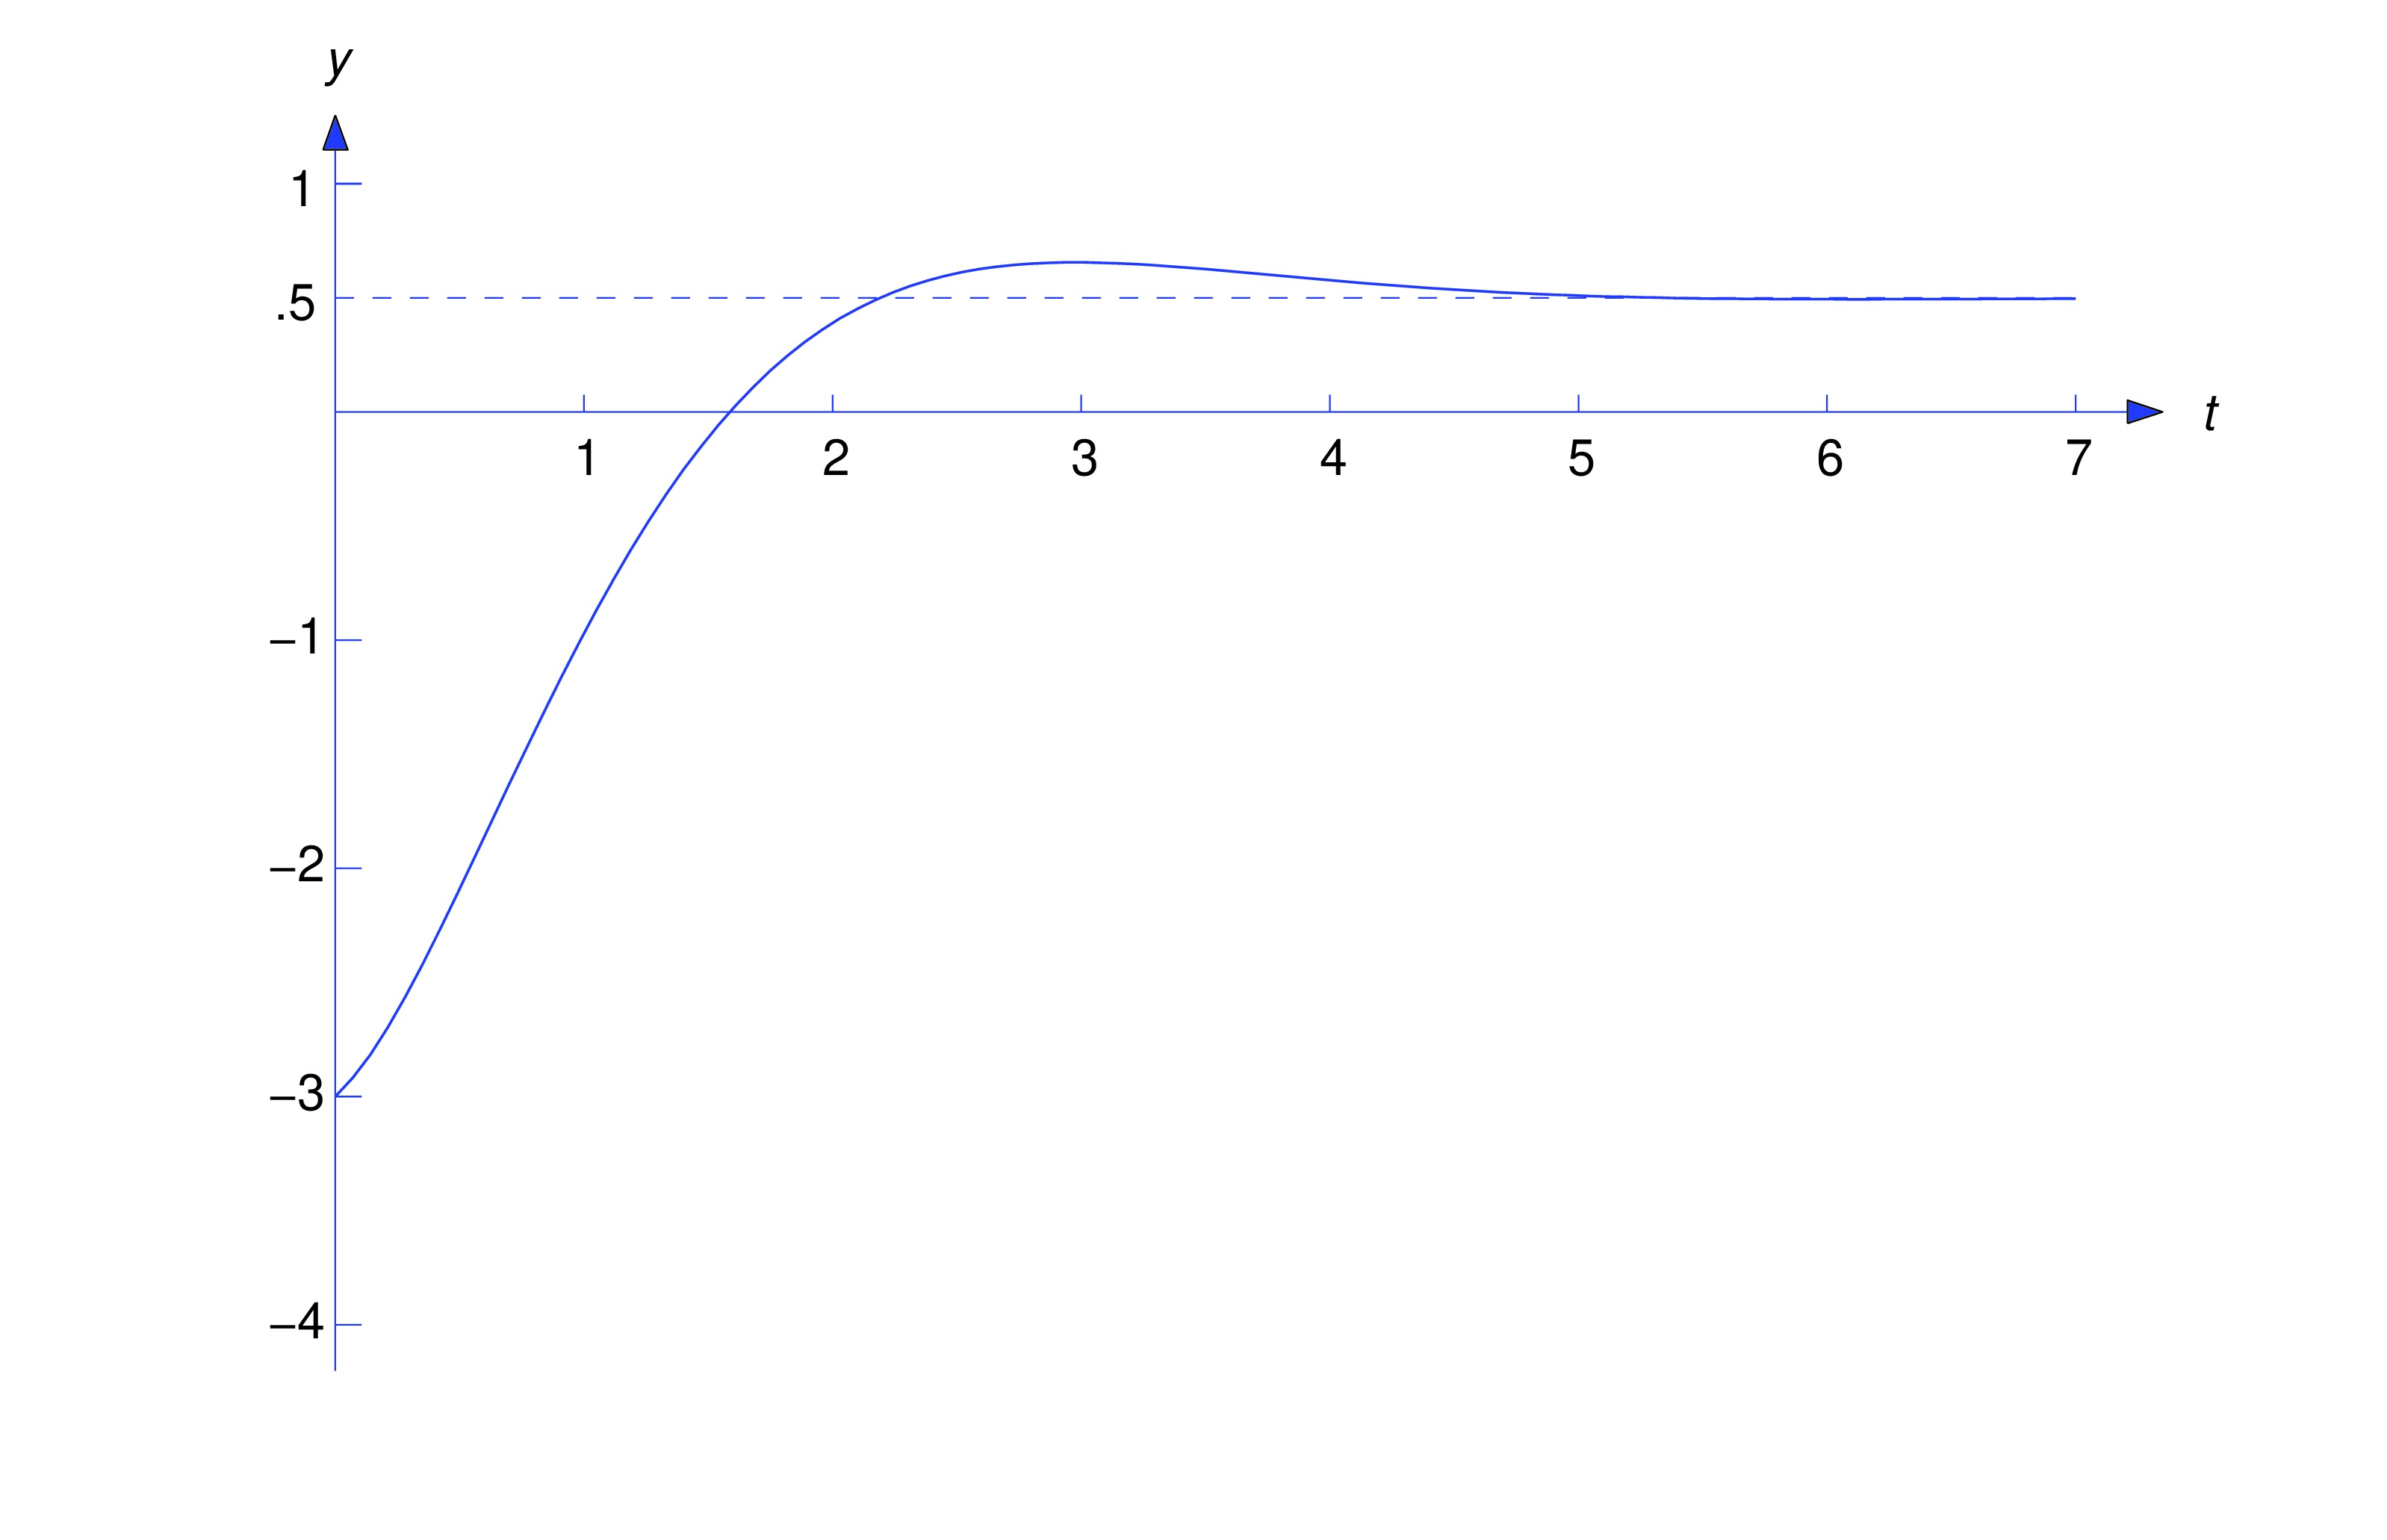
\includegraphics[bb=-78 148 689 643,width=5.67in,height=3.66in,keepaspectratio]{fig080302}}
% \caption{ $y=\dst{{1\over2}-{7\over2}e^{-t}\cos
% t-{5\over2}e^{-t}\sin t}$}
% \label{figure:8.3.2}
% \end{minipage}
% \end{figure}


\begin{example}\label{example:8.3.4}
 Solve the initial value problem
\begin{equation}\label{eq:8.3.15}
y''+2y'+2y=1, \quad   y(0)=-3,  y'(0)=1.
\end{equation}
\begin{explanation}
The characteristic polynomial is
$$
p(s)=s^2+2s+2=(s+1)^2+1
$$
and
$$
F(s)={\cal L}(1)=\frac{1}{s},
$$
so \eqref{eq:8.3.13} becomes
$$
\left[(s+1)^2+1\right] Y(s)=\frac{1}{s}+1\cdot(1-3s)+2(-3).
$$
Solving for $Y(s)$ yields
$$
Y(s)=\frac{1-s(5+3s)}{s\left[(s+1)^2+1\right]}.
$$
In Example~\ref{example:8.2.8}  we found the inverse transform of this
function to be
$$
y=\frac{1}{2}-\frac{7}{2}e^{-t}\cos t-\frac{5}{2}e^{-t}\sin t
$$
%(Figure~\ref{figure:8.3.2}),
which is therefore  the solution of  \eqref{eq:8.3.15}.

\begin{image}
 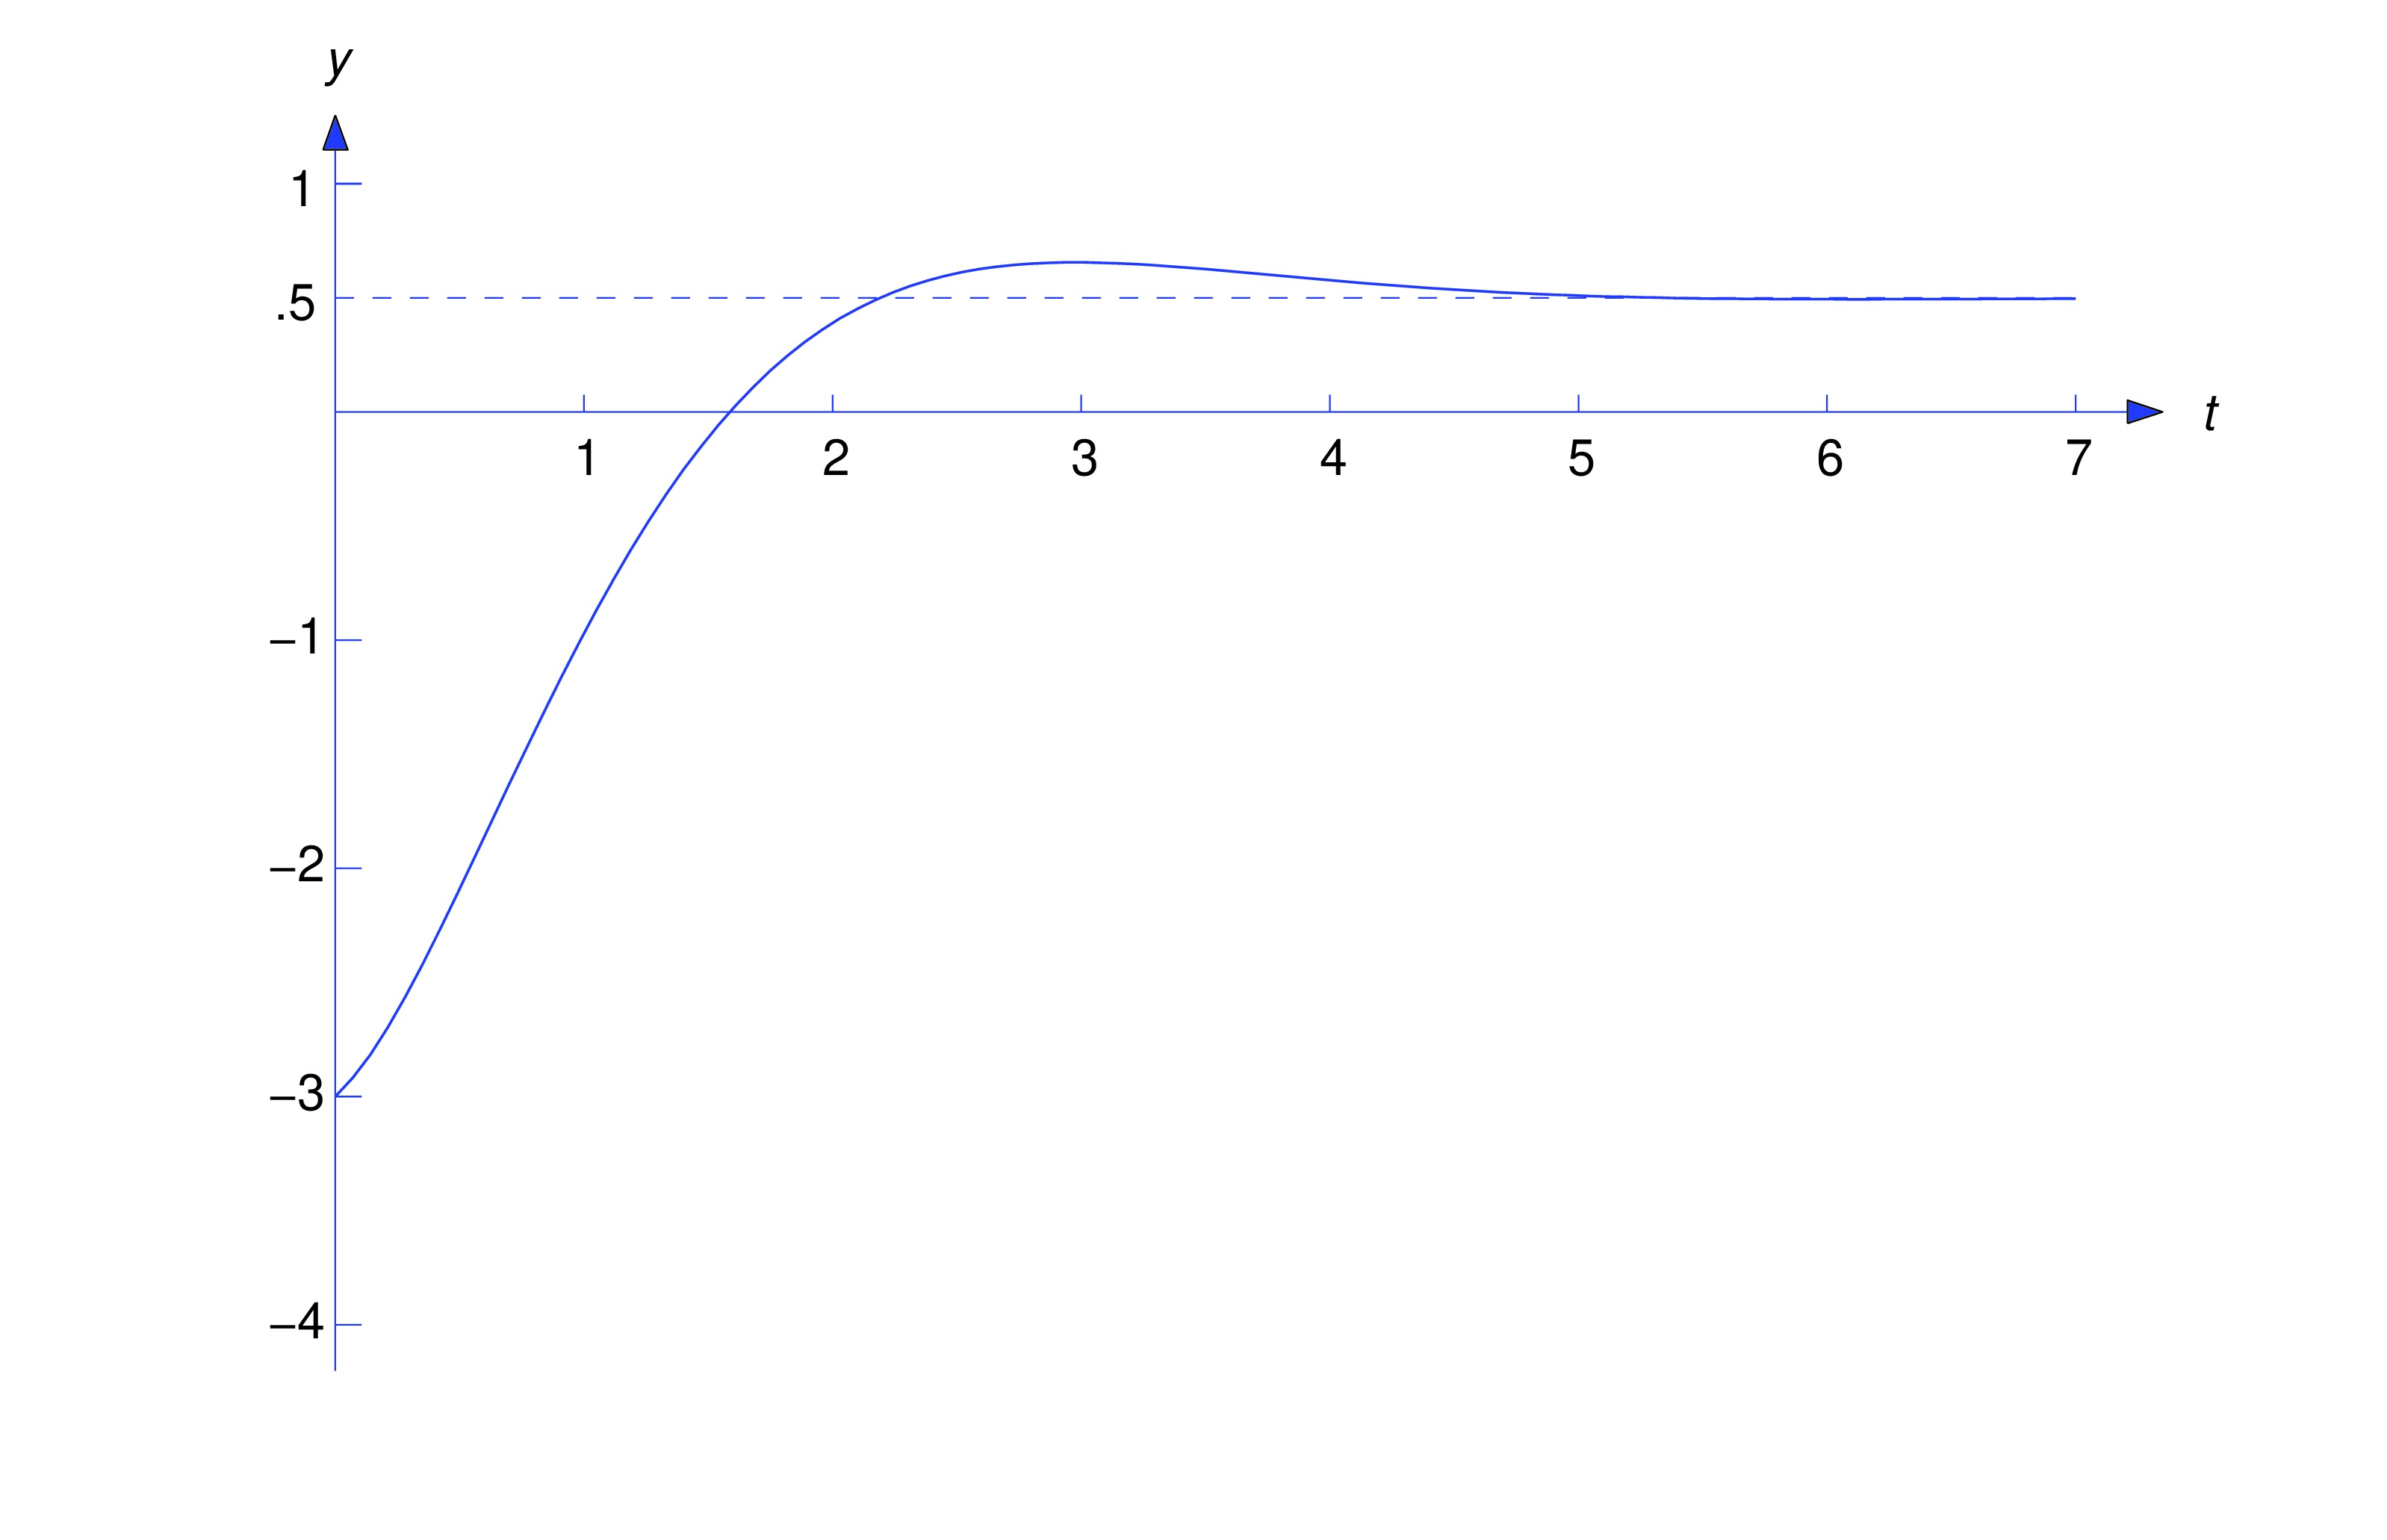
\includegraphics[height=1.5in]{fig080302.jpg}
\end{image}

\end{explanation}
\end{example}

\begin{remark}
In our examples we applied Theorems~\ref{thmtype:8.3.1} and
\ref{thmtype:8.3.2}
without verifying that the unknown function $y$ satisfies their
hypotheses. This is characteristic of the formal manipulative way in
which the Laplace transform is used to solve differential equations.
Any doubts about the validity of the method for solving a given
equation can be resolved by verifying that the resulting function $y$
is  the solution of the given problem.
\end{remark}


\section*{Text Source}
Trench, William F., "Elementary Differential Equations" (2013). Faculty Authored and Edited Books \& CDs. 8. (CC-BY-NC-SA)

\href{https://digitalcommons.trinity.edu/mono/8/}{https://digitalcommons.trinity.edu/mono/8/}


\end{document}